\chapter{CNN Architecture}

Convolutional Neural Networks (CNNs) are a special kind of multi-layer neural networks. Like almost every other neural networks they are trained with a version of the back-propagation algorithm. Where they differ is in the architecture. CNNs are designed to recognize visual patterns directly from pixel images with minimal preprocessing. They can recognize patterns with extreme variability (such as handwritten characters), and with robustness to distortions and simple geometric transformations. They are also known as shift invariant or space invariant artificial neural networks (SIANN), based on their shared-weights architecture and translation invariance characteristics.

\section{Principle}

CNNs for the most part, work by taking an input image and apply convolution operations over it with a kernel. The weights of the kernel is continuously updated over the period of training using back-propogation.

\begin{figure}
	\centering
	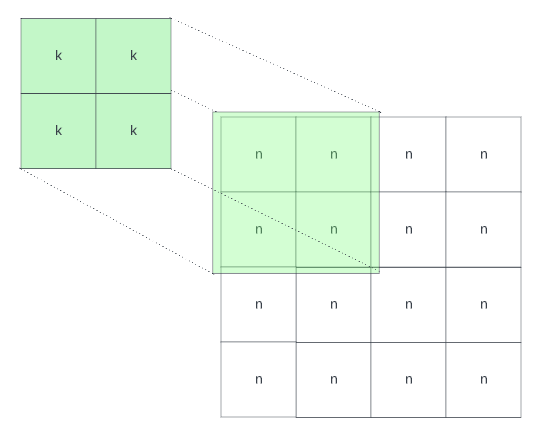
\includegraphics[width=0.5\textwidth]{images/convolution.png}
	\caption{Convolution operation}
	\label{convolution}
\end{figure}

Figure \ref{convolution} shows the convolution operation. The kernel is a matrix of weights which is applied over the input image. The kernel is slided over the image and the dot product of the kernel and the image is taken. The result of the dot product is stored in the output matrix. The kernel is slided over the image by a stride. The stride is the number of pixels by which the kernel is slided over the image. The kernel is slided over the image in both the horizontal and vertical direction. The output matrix is called the feature map. The feature map is smaller in size than the input image.

\section{PEMAN for CNN}

The PEMAN architecture can largely be used as-is for the CNN neural networks. This can be done by visualizing the CNN network in a different manner.

From the figure \ref{convolution}, we can see that the kernel values are being multiplied to the image pixel values and the output is being summed to give the output value for the feature map. This can be simplified as multiplication of weights to inputs and accumulating it to get the input. Going by this analogy, we can easily see that each convolution operation applied to the image with a kernel is a neuron. The output of each of the neuron contributes to the feature map.

By using this train of thought, we can also safely assume that PEMAN can be used for CNN architecture. The only difference is that the PEMAN architecture will not be emulating the convolution operation directly but rather, will be executing each operation inside.

The CNN process, through the previous analogy, can be distilled down to essentially a different kind of feedforward multi-layered neural network. Thus the weight updation process itself does not change except for the fact that the weights are updated for each neuron inside the convolution operation.

\section{Timing Diagram}

Since the CNN architecture is being visualized as a plain neural network, the timing diagram is different than the previous architectures. The timing diagram is shown in figure \ref{cnn_timing}

\begin{figure}
	\centering
	\includegraphics[width=\textwidth]{images/convtiming.png}
	\caption{Timing diagram for CNN}
	\label{cnn_timing}
\end{figure}

In the timing diagram, it is evident that one more dimension has been added to the number of multiplication operations, reducing the load on the accumulator even more. Thus, not only will PEMAN be able to function on CNN properly, but it will also be able to do so with more proficiency.

WHile increase in the dimension reduces the load of the accumulator, it also drastically increases the amount of operations being done in one cycle. This will lead to much lower cycles per second. This is a tradeoff that has to be made in order to implement CNN architecture on PEMAN.

To study the implementation of CNN using PEMAN, we study the same using an implementatio of the structure to predict handwritten digits from the previous dataset, the MNIST dataset.

